\newline
\newline
\vspace{3mm}
\hfill

\section{Introduction}
\hspace{2cm}In this chapter we discuss the model of our mobile robot and the low level motion control. As mentioned before our Wild Thumper is a differential drive model that takes linear and angular velocities as input, (which is different from a car-like model that takes  linear velocity and  steering angle as input). To have an appropriate and stable motion for the required velocities, low-level motion control is used to control the motion of the robot depending on the kinematics discussed below and the drivers. \\

\section{Differential Drive Robot}
\hspace{2cm}Differential Drive Robot is the simplest drive mechanism which controlled through left and right velocities (low level motion control) to move from a starting point to a global goal passing through some local goals, which called Robot Locomotion. Robot Locomotion is a mechanism of motion that describes the methods robots use to be transported from one location to another. \\
In figure \ref{fig: diff drive} , differential drive robot (is most common in two wheeled robots) has $v_r$ and $v_l$ parameters (right and left velocities respectively) which control the robot’s motion, and $R$ parameter which stands for Radius of curvature, it has two cases: \\
- The first case: Radius can be infinite, thus the angular velocity is zero resulting in a linear motion only, according to formula: $v = w * R$ \\
- The second case: If the $R$ parameter has a value which means that the robot has an angular velocity that will produce a rotation around ICR (Instantaneous Center of Rotation).\\

\begin{figure}[H]%
    \center%
    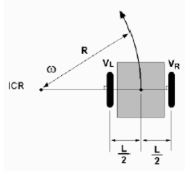
\includegraphics[width=.5\textwidth]{images/Alzahraa/differential_drive.JPG}%
     % you need to add the caption for the list of figures
    \caption[Differential Drive Robot]{The differential drive robot and its parameters}\label{fig: diff drive}%
  \end{figure}
  
%%%%%%%%%%%\figure number %%%%%%%%%%%%%%%%
Kinematics is geometric description of mechanical behavior of the robot for design and control.\cite{web001} 
The differential drive robot kinematics (forward and inverse kinematics), used in the control loop to follow the trajectory, as shown in figure \ref{fig: control loop}.

\begin{figure}[H]%
    \center%
    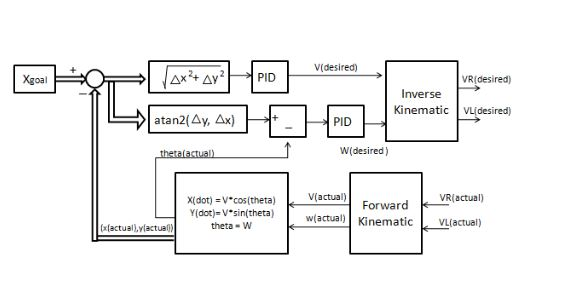
\includegraphics[width=.8\textwidth]{images/Alzahraa/control_loop.JPG}%
     % you need to add the caption for the list of figures
    \caption[Control Loop]{The control loop of differential drive robot}\label{fig: control loop}%
  \end{figure}
 
\subsection{Robot Forward kinematics}
\hspace{2cm}For differential drive robot, the linear and angular velocities are calculated using forward kinematics.
At each time instant, the right and left wheels must follow a trajectory that moves around the ICR at the same angular rate:
\begin{align*}
w(R + \frac{L}{2}) & = v_r  &  w(R - \frac{L}{2}) & = v_l
\end{align*}
 Where $L$  is the distance between any two facing wheels,$v$ is the linear velocity and $w$ is the angular velocity.
From these two equations and the formula: $v = w * R$ , the linear and angular velocities are calculated using the following equations:
\begin{align*}
v & = \frac{v_r + v_l}{2} & w & = \frac{v_r - v_l}{L}
\end{align*}
\subsection{Robot Inverse kinematics}
\hspace{2cm}Practically, to follow a specified trajectory given a new goal to be achieved described by ($x$,$y$,\(\theta)\) and the suitable values for $v$ and $w$, the required will be right and left velocities which are calculated using inverse kinematics according to the following equations:
\begin{align*}
v_r & = v + \frac{w * L}{2} & v_l & = v - \frac{w*L}{2}
\end{align*}
%
%\section{Serial communication}
%The Values of linear and angular velocities are determined by high level controller to achieve the desired goal, these values are calculated on a computer device which in our case is Nvidia Jetson Tx1 and then they are sent to Arduino using serial communication.
%sSerial is used for communication between the Arduino board and a computer or other devices. All Arduino boards have at least one serial port (also known as a UART or USART): Serial. It communicates on digital pins 0 (RX) and 1 (TX) as well as with the computer via USB. And by using Serial.read( ) function in Arduino that reads the incoming serial data, the values of both v and w is ready to be applied.\cite{web002}

\section{Low-level Motion Control}
\hspace{2cm} Control is divided into two levels, a low-level that receives $v$ and $w$ and applies the suitable voltages to motors, and a higher-level that determines the values of $v$ and $w$.
\subsection{Motor Drivers}
\hspace{2cm}Motor Driver circuits are current amplifiers. They act as a bridge between the controller and the motor in a motor drive. Motor drivers are made from discrete components which are integrated inside an IC. The input to the motor driver IC or motor driver circuit is a low current signal. The function of the circuit is to convert the low current signal to a high current signal. This high current signal is then given to the motor which helps to drive it.\cite{web003}
In robotics, To drive the robot in two opposite directions: forward and backward, H bridge is used to run the motor based on IN1 and IN2 values which are signals received from arduino and fed to the motor driver as shown in figure \ref{fig: transistor} and figure \ref{fig:possible cases}.\\
And to control the speed of DC motors, pulse width modulation pins of Arduino controller is used.
\begin{figure}[H]%
    \center%
    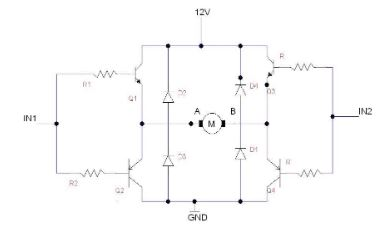
\includegraphics[width=.8\textwidth]{images/Alzahraa/H_bridge.JPG}%
     % you need to add the caption for the list of figures
    \caption[Transistor H-bridge]{Transistor Based H-Bridge Circuit\cite{web003}}\label{fig: transistor}%
  \end{figure} 
  \begin{figure}[H]%
    \center%
    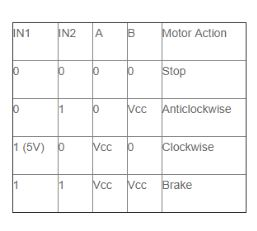
\includegraphics[width=.8\textwidth]{images/Alzahraa/possible_cases.JPG}%
     % you need to add the caption for the list of figures
    \caption[Possible Cases of Motor Driver Pins]{The four possible cases of IN1 and IN2 \cite{web003}}\label{fig:possible cases}%
  \end{figure} 
\subsection{Pulse Width Modulation}
\hspace{2cm}PWM is used to produce Analog signals from a digital device like an Arduino, to control the speed of the motors.\\
PWM signal’s values are varying from  0 to 255, 255 is the largest value that drives the motor by the maximum speed and 0 will result in stopping the motor. 
We can determine how long the motor is on and how long the motor is off according to the duty cycle percent, so if the duty cycle is 100\% this means it is fully on and if the duty cycle is 50\% this means a digital signal is on half of the time and off for the other half of the time and so on. Illustrated in figure \ref{fig:pwm} 
  \begin{figure}[H]%
    \center%
    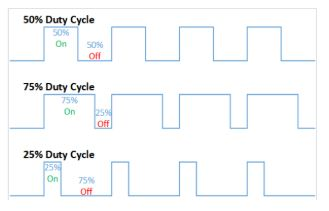
\includegraphics[width=.8\textwidth]{images/Alzahraa/duty_cycle.JPG}%
     % you need to add the caption for the list of figures
    \caption[Pulse Width Modulation]{Three scenarios of the duty cycle}\label{fig:pwm}%
  \end{figure} 
To achieve the required PWM value we map the desired voltage to its corresponding PWM signal using this relation:  \(pwm =  \frac{volt}{maximumVolt} * 255 \) then it can applied directly to the motor.

\subsection{Motors Calibration}
\hspace{2cm}Calibration is the setting or correcting of a measuring device or base level, usually by adjusting it to match or confirm to a dependably known and unvarying measure.\cite{web004}\\
In our project we calibrated the linear velocity to its corresponding value of voltage. So that for each required linear velocity, the suitable voltage will be applied. The angular velocity is calibrated from desired to actual values due to frictional force.\\
\subsubsection{Robot Linear Velocity Calibration}
\hspace{2cm}The robot is driven by Arduino code with known and equal PWM  on both sides of the robot and respectively known voltages, it moves linearly for a distance that is measured in meters and known time that is measured in seconds by a stopwatch. By using the velocity formula: \(v = \frac{s}{t}\)  linear velocities can be calculated for many values of PWM that are shown in Table \ref{table:linear_calibration}. And a polynomial function that relates the velocities to voltages can be described as:\\
For right side motors: \(V=0.2042 v^2+6.2299 v+0.4462 \)
And for left side motors: \(V=0.2047 v^2+6.2452 v+0.4473\)
The plot diagram that shows the relation between the velocity and the voltage which is limited within the recommended voltages (2-7.5) is represented in figure \ref{fig:linear calibration}
 
\begin{table}[h!]
\centering
\begin{tabular}{|c|c|c|c|c|} 
 \hline
 \multicolumn{5}{| c |}{Right Motors}\\
 \hline
 \hline
 PWM & Voltage (volts) & Distance (meters) & Time (seconds) & Velocity (m/s) \\ [0.5ex] 
 \hline\hline
 
23& 0.736& 0& 0& 0\\
30& 0.96& 2.84& 26.13& 0.1086\\
40& 1.28& 2.84& 18.49& 0.1535\\
60& 1.92& 2.84& 11.36& 0.25\\
80& 2.56& 2.84& 8.3& 0.3421\\
100& 3.2& 2.84& 6.54& 0.4342\\
120& 3.84& 2.84& 5.49& 0.5173\\
140& 4.48& 2.84& 4.19& 0.6778\\
160& 5.12& 2.84& 3.8& 0.7473\\
180& 5.76& 2.84& 3.47& 0.8184\\
200& 6.4& 2.84& 3.35& 0.8477\\
220& 7.04& 2.84& 2.75& 1.0327\\
240& 7.68& 2.84& 2.5& 1.136\\
255& 8.16& 2.84& 2.37& 1.1983 \\[1ex] 
 \hline
\end{tabular}
\end{table}

\begin{table}[h!]
\centering
\begin{tabular}{|c|c|c|c|c|}
 \hline
 \multicolumn{5}{| c |}{Left Motors}\\
 \hline
 \hline
 PWM & Voltage (volts) & Distance (meters) & Time (seconds) & Velocity (m/s) \\ [0.5ex] 
 \hline\hline
 
23& 0.7378& 0& 0& 0\\
30& 0.9623& 2.84& 26.13& 0.1086\\
40& 1.2831& 2.84& 18.49& 0.1535\\
60& 1.9247& 2.84& 11.36& 0.25\\
80& 2.5662& 2.84& 8.3& 0.3421\\
100& 3.2078& 2.84& 6.54& 0.4342\\
120& 3.8494& 2.84& 5.49& 0.5173\\
140& 4.4909& 2.84& 4.19& 0.6778\\
160& 5.1325& 2.84& 3.8& 0.7473\\
180& 5.7741& 2.84& 3.47& 0.8184\\
200& 6.4156& 2.84& 3.35& 0.8477\\
220& 7.0572& 2.84& 2.75& 1.0327\\
240& 7.6988& 2.84& 2.5& 1.136\\
255& 8.18& 2.84& 2.37& 1.1983\\[1ex] 
 \hline
\end{tabular}
\caption[Robot Linear Velocity Calibration]{Robot linear velocity calibration}
\label{table:linear_calibration}
\end{table}

\clearpage


  \begin{figure}[H]%
    \center%
    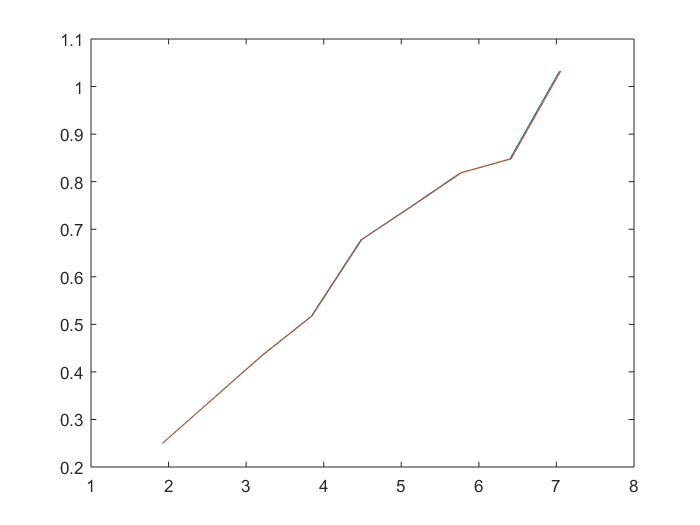
\includegraphics[width=.8\textwidth]
    {images/Alzahraa/linear_calibration.jpg}%
     % you need to add the caption for the list of figures
    \caption[Robot Linear Velocity Calibration]{The relationship between the velocity as a vertical axis and the voltage as a horizontal axis within recommended voltages}\label{fig:linear calibration}%
  \end{figure} 
  
\subsubsection{Robot Angular Velocity Calibration}
\hspace{2cm}Due to frictional force, the desired angular velocity can not be achieved by applying the right and left velocities calculated from inverse kinematics. Therefore a calibration between the desired and the actual angular velocities is required. By applying zero linear velocity with many values of angular velocities and measuring the actual for each one as shown in Table \ref{table:angular_calibration}, The relation between desired and actual angular velocities is described as: \(actual =  2 * desired + 0.55\)
\begin{table}[h!]
\centering
\begin{tabular}{|c|c|}
 \hline
 Desired Angular Velocity (rad/s) &Actual Angular Velocity (rad/s)\\ [0.5ex] 
 \hline\hline
 
0.785 & 2\\
1.57 & 3.8\\
2.355 & 5.1\\
3.14 & 6.7\\
[1ex] 
 \hline
\end{tabular}
\caption[Robot Angular Velocity Calibration]{Robot angular velocity calibration}
\label{table:angular_calibration}
\end{table}

\section{Arduino Applied Code Flow}
\hspace{2cm}The low level motion sequence is starting be receiving desired linear and angular velocities from high level controller, then apply inverse kinematic to calculate the desired right and left velocities. Then to be applied to the motors these velocities mapped to their corresponding voltages according to the previous calibration equations which finally mapped to their corresponding PWM values.\\
To recap this sequence we can consider the flowchart represented in figure \ref{fig:arduino_code}:

  \begin{figure}[H]%
    \center%
    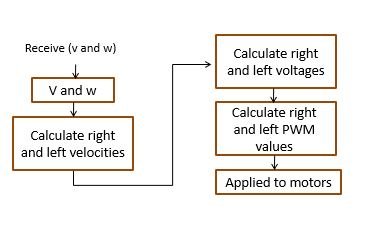
\includegraphics[width=.8\textwidth]{images/Alzahraa/flowchart.JPG}%
     % you need to add the caption for the list of figures
    \caption[Arduino Applied Code Flow]{}\label{fig:arduino_code}%
  \end{figure} 